\documentclass[conference,a4paper]{IEEEtran}
\IEEEoverridecommandlockouts

\usepackage{cite}
\usepackage{amsmath,amssymb}
\usepackage{algorithm}
\usepackage{algpseudocode}
\usepackage{graphicx}
\usepackage{booktabs}
\usepackage{tikz}
\usepackage{pgfplots}
\pgfplotsset{compat=1.18}
\usetikzlibrary{arrows.meta,matrix,positioning}
\usepackage{url}
\usepackage{xcolor}
\usepackage[colorlinks=true,urlcolor=blue,linkcolor=black,citecolor=black]{hyperref}

\begin{document}

\title{Dynamic Programming for Battery Energy Storage\\
Arbitrage Scheduling Considering\\
Capacity Degradation Cost}

\author{\IEEEauthorblockN{Made Branenda Jordhy - 13524026}
\IEEEauthorblockA{Informatics Engineering\\
School of Electrical Engineering and Informatics\\
Institut Teknologi Bandung, Ganesha 10 Bandung 40132, Indonesia\\
13524026@std.stei.itb.ac.id, ethgalleryin@gmail.com}}

\maketitle

\begin{abstract}
A battery storage owner can earn money from price arbitrage. The owner
charges the battery when electricity is cheap and discharges it when
electricity is expensive. Each charge and discharge wears the battery a
little, and this wear is a real cost. A simple buy low and sell high rule
ignores this cost and cycles the battery too much. This paper applies
dynamic programming to schedule a single battery for one day at a time. The
state is the level of charge, the stages are the hourly slots, and the
Bellman recurrence is solved by backward induction. The key idea is to add a
linear degradation cost to the reward, which keeps the problem additive and
solvable in $O(T\,N_s\,N_a)$ time. We test the method on one year of real
German day ahead prices. Scored at the real wear cost, the degradation aware
schedule earns a positive yearly profit, while a greedy rule and a dynamic
program that ignores wear both end with a loss. The method keeps about
41 percent of the gross revenue while cutting battery throughput by about
86 percent. We also confirm the linear runtime in the horizon length.
\end{abstract}

\begin{IEEEkeywords}
dynamic programming, energy storage, battery arbitrage, degradation cost,
optimal scheduling
\end{IEEEkeywords}

\section{Introduction}
Electricity prices change a lot during the day. They are often low at night
and high in the evening. A Battery Energy Storage System (BESS) can use this
change to make money. The owner buys energy and stores it when the price is
low. Later the owner sells the stored energy when the price is high. This is
called energy arbitrage.

There is a hidden cost in this plan. Every time the battery charges or
discharges, it loses a small part of its capacity. This slow loss is called
capacity fade. Over many cycles the battery becomes weaker and must be
replaced sooner. The cost of this wear is real money. A naive plan that only
looks at the price gap will cycle the battery many times. The gross revenue
looks large, but the wear cost can eat all of it and more.

This paper studies how to schedule one battery for one day. We want to
maximize the net profit, which is the revenue minus the cost of energy bought
minus the wear cost. We use dynamic programming (DP) because the problem has
the two features that DP needs. First, it has optimal substructure. The best
plan from a given hour and a given charge level depends only on the best plan
for the rest of the day. Second, it has overlapping subproblems. The same
charge level appears again and again across many possible paths.

Our main contribution is simple and clear. We put the degradation cost
directly into the reward of the DP. We use a linear cost based on energy
throughput. This keeps the reward additive and keeps the charge level as the
only state, so the standard DP still works. We then show, on real market
data, that this small change turns a losing strategy into a profitable one.
We compare three methods. The first is our DP with the wear cost. The second
is a greedy rule with no foresight. The third is a DP that ignores wear. To
be fair, we score all three with the same real wear cost. Only the wear aware
DP makes a profit.

The rest of the paper is organized as follows.
Section~\ref{sec:theory} explains the theory of dynamic programming.
Section~\ref{sec:related} reviews related work. Section~\ref{sec:problem}
states the problem. Section~\ref{sec:dp} gives the DP formulation and the
algorithm. Section~\ref{sec:baselines} describes the baselines.
Section~\ref{sec:exp} gives the data, the setup, and the results.
Section~\ref{sec:limit} lists the limits, and Section~\ref{sec:conc}
concludes.

\section{Theoretical Background}\label{sec:theory}
This section explains dynamic programming in plain terms, following the course
lecture notes~\cite{munir2026a, munir2026b}. Dynamic programming,
or DP, is a method to solve a problem by breaking it into smaller subproblems.
It solves each subproblem once and stores the answer. It then builds the answer
to the full problem from the stored answers. DP works well when a problem has
two features. The first is optimal substructure. The second is overlapping
subproblems. We explain both, then we contrast DP with the greedy method.

\subsection{Optimal Substructure}
A problem has optimal substructure when an optimal solution contains optimal
solutions to its subproblems. In our case, suppose we know the best plan for
the whole day. Take any hour $t$ and the charge level $s$ at that hour. The
part of the plan from hour $t$ to the end must itself be the best possible plan
that starts from $s$ at hour $t$. If it were not, we could swap in a better
tail and improve the whole plan, which is a contradiction. So the best plan for
a long horizon is built from the best plans for shorter horizons. This is what
lets us define a value function and solve it step by step.

\subsection{The Principle of Optimality and the Bellman Equation}
Bellman stated this idea as the principle of optimality~\cite{bellman1957}. It
says that whatever the first decision is, the remaining decisions must form an
optimal plan for the state that results from the first decision. We turn this
idea into an equation. Let $V_t(s)$ be the best total reward we can still earn
from stage $t$ when the state is $s$. The principle gives a recurrence,
\begin{equation}
V_t(s) = \max_{a}\big[\, R_t(s,a) + V_{t+1}(\,\mathrm{next}(s,a)\,) \,\big].
\label{eq:bellman-general}
\end{equation}
The term $R_t(s,a)$ is the reward of taking action $a$ now. The term
$V_{t+1}(\cdot)$ is the best reward for the rest of the horizon. We add them and
take the action that gives the most. This single equation is the heart of DP.
We solve it from the last stage back to the first. This order is called
backward induction. We fill a table of values, one cell per state per stage.
Because we go backward, the future values we need are always ready.

\subsection{Overlapping Subproblems}
A problem has overlapping subproblems when the same subproblem appears many
times. If we solved the recurrence by plain recursion, we would compute the
same $V_t(s)$ again and again. Fig.~\ref{fig:subproblems} shows why. Starting
from one state, the recursion branches into actions, and different branches
soon reach the same state at the same stage. The number of distinct states is
small and bounded, but the number of paths grows fast. DP avoids the waste. It
stores each $V_t(s)$ in a table and reads it back when needed. So each
subproblem is solved only once. This turns an exponential search over paths
into a loop over a small table.

\begin{figure}[t]
\centering
% Overlapping subproblems. A naive recursion on the value function expands the
% same state many times. Here we show the recursion for V_t(s) as a tree. Nodes
% with the same (stage, SoC) label, shaded the same color, are the same
% subproblem. A table stores each one so it is solved only once.
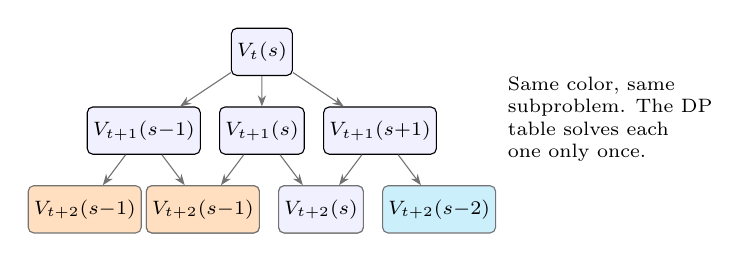
\begin{tikzpicture}[
    level distance=10mm,
    sibling distance=15mm,
    every node/.style={font=\scriptsize},
    sub/.style={draw, rounded corners=2pt, inner sep=2pt, minimum size=6mm},
    rep/.style={sub, fill=orange!25},
    repb/.style={sub, fill=cyan!20},
    norm/.style={sub, fill=blue!6},
    edge from parent/.style={draw, black!55, -{Stealth[length=4pt]}},
]
\node[norm] {$V_t(s)$}
  child {node[norm] {$V_{t+1}(s{-}1)$}
    child {node[rep] {$V_{t+2}(s{-}1)$}}
    child {node[repb] {$V_{t+2}(s{-}2)$}}
  }
  child {node[norm] {$V_{t+1}(s)$}
    child {node[rep] {$V_{t+2}(s{-}1)$}}
    child {node[norm] {$V_{t+2}(s)$}}
  }
  child {node[norm] {$V_{t+1}(s{+}1)$}
    child {node[norm] {$V_{t+2}(s)$}}
    child {node[repb] {$V_{t+2}(s{-}2)$}}
  };
% Note about the repeats.
\node[font=\scriptsize, align=left, anchor=north west]
  at (3.0,-0.2) {Same color, same\\subproblem. The DP\\table solves each\\one only once.};
\end{tikzpicture}

\caption{Overlapping subproblems in the value recursion. A plain recursion
reaches the same state at the same stage along different branches. Nodes with
the same color are the same subproblem. The DP table stores each one once, so
the work drops from a search over paths to a loop over states.}
\label{fig:subproblems}
\end{figure}

\subsection{Why Not Greedy}
A greedy method makes the choice that looks best right now and never looks
back. Greedy is fast and simple. It is correct only for special problems where
a local best choice is always part of a global best plan. Battery arbitrage is
not such a problem. The best action in one hour depends on prices in later
hours and on the wear cost over the whole day. A greedy rule that sells at the
first high price may miss a higher price later, or it may cycle the battery for
a small gain that the wear cost wipes out. DP looks at the whole horizon at
once through the value function, so it does not fall into these traps. This is
the main reason we choose DP for this problem, and the experiments in
Section~\ref{sec:exp} show the gap in real money.

\section{Related Work}\label{sec:related}
Dynamic programming is a classic method for sequential decisions
\cite{bellman1957}. Standard algorithm textbooks present it as a way to solve
problems with optimal substructure and overlapping subproblems
\cite{kleinberg2006}. Battery arbitrage is a natural fit because the decision
in each slot depends on the charge level, which is a small and bounded state.

Several works study battery scheduling in electricity markets. Jiang and
Powell use approximate dynamic programming for hour ahead bidding with storage
in the real time market \cite{jiang2015}. Other works frame arbitrage as a
linear or mixed integer program and add operational limits or revenue stacking
\cite{revenuestack2023}. Some works include market impact and solve the
problem with dynamic programming for a price maker \cite{energy2021}. Recent
work studies arbitrage profit when efficiency and degradation both change over
time, and uses linear and nonlinear programs \cite{jes2024}.

Our work is smaller in scope but clear in message. We keep the model simple
and exact. We use a plain backward induction over a discrete charge level. We
focus on one teaching point. A small additive wear term inside the reward is
enough to fix the over cycling problem, and the method stays in the basic DP
form taught in an algorithms course.

\section{Problem Statement}\label{sec:problem}
We schedule one battery over one day. The day has $T$ time slots. Each slot
lasts $\Delta t$ hours. In this study $T=24$ and $\Delta t = 1$ hour. The
price in slot $t$ is $p_t$ in EUR per MWh. We assume the prices are known in
advance. This is the perfect foresight case, which is common as a first model.

The battery has a usable energy capacity $E_{\max}$ in MWh. It has a charge
power limit $P_{\text{chg}}^{\max}$ and a discharge power limit
$P_{\text{dis}}^{\max}$, both in MW. So the most energy that can move in one
slot is the power limit times $\Delta t$. The battery has a round trip
efficiency $\eta$ between 0 and 1. We split it into a one way efficiency
$\eta_1 = \sqrt{\eta}$ for charge and the same for discharge.

The state of charge (SoC) is the energy stored in the battery. We write it as
$s$. The action in each slot moves energy in or out. We use a simple energy
rule. When charging by an SoC amount $g$, the grid energy bought is
$g/\eta_1$. When discharging by an SoC amount $h$, the grid energy sold is
$\eta_1 h$. The SoC update is
\begin{align}
\text{charge:}\quad & s_{t+1} = s_t + g_t,\\
\text{discharge:}\quad & s_{t+1} = s_t - h_t,\\
\text{idle:}\quad & s_{t+1} = s_t,
\end{align}
with the SoC kept in $[0, E_{\max}]$ at all times.

We want to maximize the net profit over the day,
\begin{equation}
\begin{aligned}
\text{profit} = \sum_{t=0}^{T-1}\Big[\,
& p_t\,(\text{energy sold})_t\\[-2pt]
& - p_t\,(\text{energy bought})_t - C_{\text{deg}}(a_t) \,\Big],
\end{aligned}
\end{equation}
subject to the SoC dynamics and the power limits. Here $a_t$ is the action in
slot $t$ and $C_{\text{deg}}$ is the wear cost of that action.

\section{Dynamic Programming Formulation}\label{sec:dp}

\subsection{State, Stage, and Action}
The stage is the time index $t$, from $0$ to $T$. The state is the SoC. We
make the SoC discrete. We split the range $[0, E_{\max}]$ into $N_s$ equal
levels. The step size is $\delta = E_{\max}/(N_s-1)$. A state is the index of
a level. The action in slot $t$ is the choice of the next SoC level. The
change in level fixes the charge or discharge energy. The power limits set how
many levels we can move up or down in one slot. So the action set in each
state is a small window of nearby levels. We call its size $N_a$. Because we
pick the next level on the grid, every transition lands exactly on a grid
point. We do not need any interpolation. Fig.~\ref{fig:lattice} shows the
idea.

\begin{figure}[t]
\centering
% Conceptual DP state and transition lattice.
% Stages t on the x axis, discrete SoC levels on the y axis. From one state a
% few actions lead to nearby SoC levels: charge moves up, discharge moves down,
% idle stays level. Only a small grid is drawn for clarity.
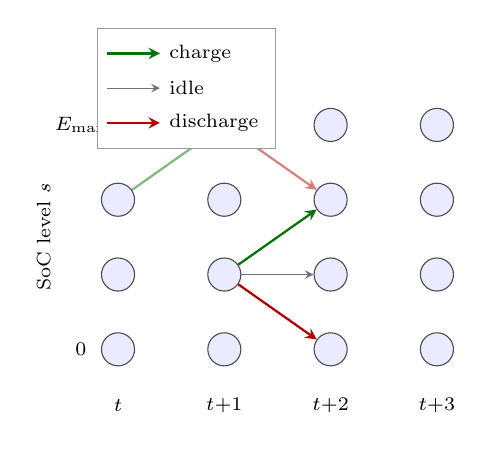
\begin{tikzpicture}[
    x=1.35cm, y=0.95cm,
    node distance=0pt,
    state/.style={circle, draw=black!70, fill=blue!8, minimum size=4.2mm,
                  inner sep=0pt, font=\scriptsize},
    chg/.style={->, >=stealth, green!45!black, thick},
    dis/.style={->, >=stealth, red!70!black, thick},
    idle/.style={->, >=stealth, black!55},
]
% Grid of states: 4 stages, 4 SoC levels.
\foreach \t in {0,1,2,3} {
  \foreach \s in {0,1,2,3} {
    \node[state] (n\t\s) at (\t,\s) {};
  }
}
% Stage labels.
\foreach \t/\lab in {0/{$t$},1/{$t{+}1$},2/{$t{+}2$},3/{$t{+}3$}} {
  \node[font=\scriptsize] at (\t,-0.75) {\lab};
}
% SoC axis label.
\node[rotate=90, font=\scriptsize] at (-0.7,1.5) {SoC level $s$};
\node[font=\scriptsize] at (-0.35,0) {$0$};
\node[font=\scriptsize] at (-0.35,3) {$E_{\max}$};

% Sample transitions out of state (n11): charge up, idle, discharge down.
\draw[chg]  (n11) -- (n22);
\draw[idle] (n11) -- (n21);
\draw[dis]  (n11) -- (n20);
% A couple more to suggest the full fan-out.
\draw[chg, opacity=0.5]  (n02) -- (n13);
\draw[dis, opacity=0.5]  (n13) -- (n22);

% Legend.
\matrix[draw=black!40, fill=white, inner sep=3pt, row sep=1pt,
        anchor=north west, font=\scriptsize] at (-0.2,4.3) {
  \draw[chg] (0,0) -- (0.5,0); & \node[anchor=west] {charge}; \\
  \draw[idle] (0,0) -- (0.5,0); & \node[anchor=west] {idle}; \\
  \draw[dis] (0,0) -- (0.5,0); & \node[anchor=west] {discharge}; \\
};
\end{tikzpicture}

\caption{The DP state and transition lattice. Stages run left to right.
Discrete SoC levels run bottom to top. From one state, charging moves up,
discharging moves down, and idle stays level. The power limit bounds how far a
single step can move.}
\label{fig:lattice}
\end{figure}

\subsection{Reward}
The reward of a transition is the money it earns in that slot. Let the change
in SoC be $\Delta = s' - s$. If $\Delta>0$ the battery charges, so it buys
$\Delta/\eta_1$ units of energy and the price effect is $-p_t\,\Delta/\eta_1$.
If $\Delta<0$ the battery discharges by $|\Delta|$, so it sells
$\eta_1|\Delta|$ units and the price effect is $+p_t\,\eta_1|\Delta|$. We then
subtract the wear cost. The reward is
\begin{equation}
R_t(s,s') = (\text{price effect}) - c_{\text{deg}}\,\big(g + h\big),
\end{equation}
where $g$ and $h$ are the charge and discharge amounts on the SoC side, and at
most one of them is nonzero in a slot.

\subsection{Degradation Cost}
The wear cost is the heart of this paper. We use a linear throughput model,
\begin{equation}
C_{\text{deg}}(a) = c_{\text{deg}}\,(g + h).
\label{eq:deg}
\end{equation}
The term $g+h$ is the energy that moves through the battery in that slot on the
SoC side. The factor $c_{\text{deg}}$ is the marginal wear cost per MWh of
throughput. We get it from the battery capital cost divided by the total
energy the battery can move over its life. This model has two good properties.
It is additive over slots, and it depends only on the current action. So it
fits the DP with the SoC as the only state, and it does not break the Markov
property.

\subsection{Bellman Recurrence and Backward Induction}
Let $V_t(s)$ be the best profit we can still earn from stage $t$ with SoC
level $s$. The recurrence is
\begin{equation}
V_t(s) = \max_{s' \in \mathcal{A}(s)} \big[\, R_t(s,s') + V_{t+1}(s') \,\big],
\label{eq:bellman}
\end{equation}
where $\mathcal{A}(s)$ is the set of feasible next levels under the power
limits. The terminal value is
\begin{equation}
V_T(s) = \begin{cases} 0 & \text{if } s \ge s_{\min}^{\text{end}},\\
-\infty & \text{otherwise.} \end{cases}
\end{equation}
We require the end SoC to be at least a set minimum. This stops the solver
from draining the battery for free at the end of the day. We solve the
recurrence by backward induction. We fill the table from $t=T$ down to $t=0$.
Fig.~\ref{fig:backward} shows one step. We store the best next level in a
policy table. Then we walk forward from the start SoC and read the policy
table to rebuild the schedule. Algorithm~\ref{alg:dp} gives the full method.

\begin{figure}[t]
\centering
% Backward induction step. The value of a state at stage t is computed from the
% already known values at stage t+1. We take the best over the feasible actions.
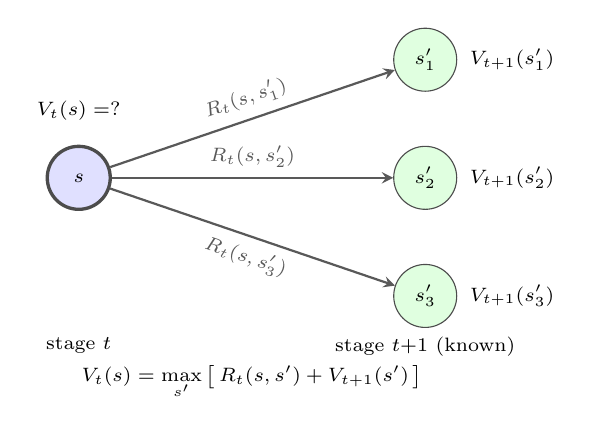
\begin{tikzpicture}[
    x=2.2cm, y=1.0cm,
    state/.style={circle, draw=black!70, minimum size=8mm, inner sep=0pt,
                  font=\scriptsize},
    known/.style={state, fill=green!12},
    cur/.style={state, fill=blue!12, very thick},
    arr/.style={->, >=stealth, thick, black!65},
]
% Stage t (current, unknown) on the left, stage t+1 (known) on the right.
\node[cur] (s) at (0,1.5) {$s$};
\node[known] (a) at (2,3) {$s'_1$};
\node[known] (b) at (2,1.5) {$s'_2$};
\node[known] (c) at (2,0) {$s'_3$};

\node[font=\scriptsize, above] at (0,2.1) {$V_t(s)=?$};
\node[font=\scriptsize, right=1pt] at (a.east) {$V_{t+1}(s'_1)$};
\node[font=\scriptsize, right=1pt] at (b.east) {$V_{t+1}(s'_2)$};
\node[font=\scriptsize, right=1pt] at (c.east) {$V_{t+1}(s'_3)$};

\draw[arr] (s) -- node[above, font=\scriptsize, sloped] {$R_t(s,s'_1)$} (a);
\draw[arr] (s) -- node[above, font=\scriptsize] {$R_t(s,s'_2)$} (b);
\draw[arr] (s) -- node[below, font=\scriptsize, sloped] {$R_t(s,s'_3)$} (c);

\node[font=\scriptsize] at (1,-1.1)
  {$V_t(s)=\max\limits_{s'}\big[\,R_t(s,s')+V_{t+1}(s')\,\big]$};

\node[font=\scriptsize, anchor=north] at (0,-0.4) {stage $t$};
\node[font=\scriptsize, anchor=north] at (2,-0.4) {stage $t{+}1$ (known)};
\end{tikzpicture}

\caption{One backward induction step. The values at stage $t{+}1$ are already
known. The value at stage $t$ is the best over the feasible actions of the
slot reward plus the known future value.}
\label{fig:backward}
\end{figure}

\begin{algorithm}[t]
\caption{Battery arbitrage by dynamic programming}
\label{alg:dp}
\begin{algorithmic}[1]
\State \textbf{Input:} prices $p_{0..T-1}$, battery params, $N_s$,
start level $s_0$, end minimum $s_{\min}^{\text{end}}$
\State \textbf{Output:} optimal schedule and net profit
\For{$s = 0$ to $N_s-1$}
  \State $V_T(s) \gets 0$ if $s \ge s_{\min}^{\text{end}}$ else $-\infty$
\EndFor
\For{$t = T-1$ down to $0$}
  \For{$s = 0$ to $N_s-1$}
    \State $V_t(s) \gets -\infty$
    \For{$s'$ in feasible window of $s$}
      \State $v \gets R_t(s,s') + V_{t+1}(s')$
      \If{$v > V_t(s)$}
        \State $V_t(s) \gets v$,\quad $P_t(s) \gets s'$
      \EndIf
    \EndFor
  \EndFor
\EndFor
\State $s \gets s_0$
\For{$t = 0$ to $T-1$}
  \State record action from $s$ to $P_t(s)$,\quad $s \gets P_t(s)$
\EndFor
\end{algorithmic}
\end{algorithm}

\subsection{Complexity}
For each stage we loop over $N_s$ states. For each state we loop over $N_a$
feasible next levels. So one stage costs $O(N_s\,N_a)$. Over $T$ stages the
total cost is
\begin{equation}
O(T\,N_s\,N_a).
\end{equation}
This is linear in the horizon length and linear in the number of states. The
window size $N_a$ comes from the power limit. If the power limit is a fixed
fraction of the capacity, then $N_a$ grows with $N_s$, so the cost grows like
$O(T\,N_s^2)$ as the grid gets finer. We check both effects in the
experiments.

\subsection{A Small Worked Example}
A tiny example shows how the table fills. Take a battery with $E_{\max}=1$ MWh
and three SoC levels, so the levels are $0$, $0.5$, and $1.0$ MWh. Let the
power limit allow a move of one level per slot. Set the efficiency to one and
the wear cost to zero, to keep the numbers clean. Take three slots with prices
$p_0=10$, $p_1=50$, and $p_2=20$ EUR per MWh. The terminal value is
$V_3(s)=0$ for every level.

We work backward. In slot $t=2$ at price $20$, from the middle level the best
move is to hold, since selling at $20$ first needs the battery to have charged
earlier. The values become $V_2(0)=0$, $V_2(0.5)=0$, and $V_2(1.0)=0$ for the
hold action, while a sell at this low price is not yet useful on its own. In
slot $t=1$ at the high price $50$, selling is very good. From the full level we
can sell $0.5$ MWh and earn $50 \times 0.5 = 25$. So $V_1(1.0)=25$ and the
best action is to discharge. From the middle level we can also sell and reach
$V_1(0.5)=25$ if it was reached with stored energy. In slot $t=0$ at the low
price $10$, buying is cheap. From the empty level we can charge $0.5$ MWh at a
cost of $10 \times 0.5 = 5$, move to the middle level, and then collect the
future value. The recurrence in~\eqref{eq:bellman} picks the buy now and sell
later path. The policy table stores these moves. The forward walk then reads
the table and returns the schedule. This is the same buy low and sell high
logic, but the DP finds it by global search, not by a local rule.

Fig.~\ref{fig:vtable} shows the real value table for one day from our solver.
Each column is a stage and each row is an SoC level. The color is the value to
go $V_t(s)$, the best profit still possible from that cell. The black line is
the optimal path that the forward walk rebuilds from the policy table. The path
charges to a high SoC in the cheap morning, holds, then discharges into the
expensive hours. This is the DP table filled with real numbers.

\begin{figure}[t]
\centering

\includegraphics[width=\columnwidth]{figures/fig_vtable.png}
\caption{The DP value table for one example day. The horizontal axis is the
stage $t$. The vertical axis is the SoC level. The color is the value to go
$V_t(s)$. The black line is the optimal path rebuilt from the policy table. It
charges in the cheap hours and discharges in the costly ones.}
\label{fig:vtable}
\end{figure}

\section{Baseline Methods}\label{sec:baselines}
We compare the DP against two baselines.

The first baseline is a greedy threshold rule. It looks at the price in the
current slot only. If the price is below a low threshold, it charges as much
as the power limit and the free space allow. If the price is above a high
threshold, it discharges as much as allowed. Otherwise it stays idle. The two
thresholds are price quantiles of the same day. We use the 30th and the 70th
percentile. This rule is myopic. It has no foresight and it ignores the wear
cost when it decides.

The second baseline is a DP that ignores wear. It is the same solver as in
Section~\ref{sec:dp}, but with $c_{\text{deg}}=0$ in the planning reward. This
isolates the effect of the wear term. It shows what happens when we plan only
for gross revenue.

To compare the three methods in a fair way, we score all of them with the same
real wear cost. Each method picks its own actions. Then we charge every
schedule the same real cost per MWh of throughput. This gives a true net
profit for each method, even for the method that ignored wear when it planned.

\section{Experiments and Results}\label{sec:exp}

\subsection{Data}
We use real day ahead electricity prices from Open Power System Data
\cite{opsd}. We take the German and Luxembourg bidding zone for the calendar
year 2019. The prices are hourly and in EUR per MWh. We keep only full days
with all 24 hours present, which gives 364 days. The mean price is about
37.7 EUR per MWh. The mean daily spread between the highest and lowest hour is
about 30.2 EUR per MWh. Some hours have negative prices, which is a real
feature of this market when supply is high. A Python script downloads the data
and reshapes it into one row per day. The C++ solver reads this file.
Fig.~\ref{fig:price} shows the data. The left panel is the mean price for each
hour of the day. It has the typical shape, low at night and two peaks, one in
the morning and a larger one in the evening. This shape is what arbitrage
exploits. The right panel is the price for every day and hour of the year. The
red bands at the morning and evening hours are the expensive times. The few
blue marks are the negative price hours.

\begin{figure}[t]
\centering

\includegraphics[width=\columnwidth]{figures/fig_price_context.png}
\caption{The price data for 2019. Left: the mean price by hour of day, with a
band for the 25th to 75th percentile. The double peak shape is what arbitrage
uses. Right: a heatmap of price by day and hour over the year. Red is
expensive, blue is the rare negative price.}
\label{fig:price}
\end{figure}

\subsection{Setup}
We use a normalized battery of $E_{\max}=1$ MWh. The charge and discharge power
limits are both 0.5 MW, which is a 0.5 C rate. The round trip efficiency is
$\eta = 0.86$. The real wear cost is $c_{\text{deg}}=12$ EUR per MWh of
throughput, which is in the range used in storage studies. The battery starts
each day half full and must end at least half full. The DP uses $N_s=101$ SoC
levels in the main runs. The solver is written in C++17. We run four
experiments.

\subsection{E1: Main Comparison}
Table~\ref{tab:e1} shows the yearly totals for the three methods, all scored
at the real wear cost. The result is clear. The wear aware DP earns a positive
yearly true net profit of about 1390 EUR. The greedy rule and the wear blind
DP both end with a loss. The wear blind DP earns the largest gross revenue,
about 8645 EUR, but it cycles the battery 648 times in the year. The wear cost
of all that cycling is larger than the revenue, so the true net is about
$-6925$ EUR. The greedy rule sits in the middle and still loses money.

\begin{table}[t]
\caption{E1: yearly totals over 364 days, scored at the real wear cost
$c_{\text{deg}}=12$ EUR/MWh. Best true net profit in bold.}
\label{tab:e1}
\centering
\small
\begin{tabular}{lrrrr}
\toprule
Method & True net & Gross & Wear cost & Cycles\\
       & (EUR) & (EUR) & (EUR) & \\
\midrule
DP with wear (ours) & \textbf{1389.6} & 3555.6 & 2166.0 & 90.3\\
DP without wear     & $-6924.7$ & 8645.3 & 15570.0 & 648.8\\
Greedy threshold    & $-4996.6$ & 6397.4 & 11394.0 & 474.8\\
\bottomrule
\end{tabular}
\end{table}

The trade is easy to read. The wear aware DP keeps about 41 percent of the
gross revenue of the wear blind DP. At the same time it cuts the battery
throughput by about 86 percent. It gives up some gross revenue but saves much
more in wear, so the net profit is higher. This is the central result of the
paper.

Fig.~\ref{fig:headtohead} shows why foresight matters, using the greedy rule
and the DP on the same day. The greedy rule sells at the first high prices in
the morning, so the battery is empty by the time the largest evening peak
arrives. The DP holds its energy and sells into that evening peak instead. Both
use one full cycle on this day, but the DP earns more because it places the
same energy at a better time. The plan that looks ahead wins.

\begin{figure*}[t]
\centering

\includegraphics[width=0.86\textwidth]{figures/fig_headtohead.png}
\caption{Greedy rule versus dynamic programming on the same day. Blue is the
price, red is the SoC, green bars are the net action. The greedy rule sells too
early and misses the largest evening peak. The DP holds its energy and sells
into that peak, so it earns more from the same single cycle.}
\label{fig:headtohead}
\end{figure*}

Fig.~\ref{fig:example} shows one example day. The DP charges in the cheap
early morning hours and discharges into the two evening price peaks. It does
not cycle on small price gaps because the wear cost is not worth it. The SoC
path stays smooth and uses only a few clean cycles.

\begin{figure}[t]
\centering
% Example day: price curve, optimal SoC path, and charge/discharge actions.
% Data: figures/example_day.csv (from the C++ DP solver, real 2019-01-24 prices).
% Two stacked axes share the same frame. The left axis shows the SoC and the
% action. The right axis shows the price. We give the right axis label its own
% room with ylabel near ticks so the two y labels do not overlap.
\begin{tikzpicture}
% Left axis: SoC and net action bars.
\begin{axis}[
    name=axsoc,
    width=0.80\columnwidth,
    height=5.0cm,
    xlabel={Hour of day},
    ylabel={SoC and action (MWh)},
    xmin=-0.5, xmax=23.5,
    xtick={0,4,8,12,16,20,23},
    ymin=-0.6, ymax=1.15,
    ytick={-0.5,0,0.5,1.0},
    axis y line*=left,
    axis x line=bottom,
    ylabel near ticks,
    enlarge x limits=false,
    tick label style={font=\scriptsize},
    label style={font=\scriptsize},
    legend style={font=\scriptsize, at={(0.02,0.98)}, anchor=north west,
                  draw=none, fill=white, fill opacity=0.75, text opacity=1},
]
\addplot[ybar, bar width=5pt, fill=green!55!black, draw=green!40!black,
         fill opacity=0.6]
    table[col sep=comma, x=hour, y=net_action] {figures/example_day.csv};
\addlegendentry{Charge (+) / Discharge (-)}
\addplot[red, thick, mark=square*, mark size=1pt]
    table[col sep=comma, x=hour, y=soc] {figures/example_day.csv};
\addlegendentry{SoC}
\end{axis}

% Right axis: price. Same frame, only the right y axis is drawn.
\begin{axis}[
    width=0.80\columnwidth,
    height=5.0cm,
    at={(axsoc.south east)}, anchor=south east,
    xmin=-0.5, xmax=23.5,
    ymin=40, ymax=130,
    axis y line*=right,
    axis x line=none,
    ylabel={Price (EUR/MWh)},
    ylabel near ticks,
    tick label style={font=\scriptsize},
    label style={font=\scriptsize},
    legend style={font=\scriptsize, at={(0.98,0.02)}, anchor=south east,
                  draw=none, fill=white, fill opacity=0.75, text opacity=1},
]
\addplot[blue, thick, mark=*, mark size=1pt]
    table[col sep=comma, x=hour, y=price] {figures/example_day.csv};
\addlegendentry{Price}
\end{axis}
\end{tikzpicture}

\caption{One example day with the wear aware DP. The blue line is the price on
the left axis. The red squares are the SoC on the right axis. The green bars
are the net action, positive for charge and negative for discharge. The
battery charges in the cheap trough and discharges into the price peaks.}
\label{fig:example}
\end{figure}

\subsection{E2: Sensitivity to the Wear Cost}
In this experiment we keep the real wear cost fixed at 12 EUR per MWh. We only
change the wear cost that the DP plans with. We then score the schedule at the
real cost. Fig.~\ref{fig:e2} shows the result. When the planned cost is too
low, the DP cycles too much and the true net is low or negative. When the
planned cost is too high, the DP is too shy and gives up good trades. The best
true net is reached when the planned cost equals the real cost of 12 EUR per
MWh. This matches the theory. The number of yearly cycles falls in a smooth
way as the planned cost rises. This shows that the wear term is a clean knob
that trades revenue for fewer cycles.

\begin{figure}[t]
\centering
% E2: sensitivity to the planned degradation cost.
% Left axis: yearly true net profit (scored at the real cost).
% Right axis: yearly equivalent full cycles.
% Data: figures/e2_cdeg_sweep.csv
% Two stacked axes share the same frame. ylabel near ticks keeps each y label
% close to its own axis so the left and right labels do not overlap.
\begin{tikzpicture}
\begin{axis}[
    name=axnet,
    width=0.80\columnwidth,
    height=5.2cm,
    xlabel={Planned degradation cost (EUR/MWh)},
    ylabel={Yearly true net profit (EUR)},
    xmin=0, xmax=30,
    axis y line*=left,
    ylabel near ticks,
    tick label style={font=\scriptsize},
    label style={font=\scriptsize},
    legend style={font=\scriptsize, at={(0.97,0.55)}, anchor=east,
                  draw=none, fill=white, fill opacity=0.75, text opacity=1},
]
\addplot[blue, thick, mark=*, mark size=1.3pt]
    table[col sep=comma, x=plan_c_deg, y=true_net] {figures/e2_cdeg_sweep.csv};
\addlegendentry{True net profit}
% Mark the real cost c_deg = 12 with a vertical line.
\addplot[gray, dashed, thick] coordinates {(12,-7000) (12,2000)};
\end{axis}
\begin{axis}[
    width=0.80\columnwidth,
    height=5.2cm,
    at={(axnet.south east)}, anchor=south east,
    xmin=0, xmax=30,
    axis y line*=right,
    axis x line=none,
    ylabel={Yearly full cycles},
    ylabel near ticks,
    tick label style={font=\scriptsize},
    label style={font=\scriptsize},
    legend style={font=\scriptsize, at={(0.97,0.33)}, anchor=east,
                  draw=none, fill=white, fill opacity=0.75, text opacity=1},
]
\addplot[red, thick, mark=square*, mark size=1.3pt]
    table[col sep=comma, x=plan_c_deg, y=total_cycles] {figures/e2_cdeg_sweep.csv};
\addlegendentry{Full cycles}
\end{axis}
\end{tikzpicture}

\caption{E2: effect of the planned wear cost. The blue line is the yearly
true net profit on the left axis. The red line is the yearly number of full
cycles on the right axis. The dashed vertical line marks the real wear cost of
12 EUR per MWh, where the true net is highest.}
\label{fig:e2}
\end{figure}

\subsection{E3: Discretization Granularity}
We vary the number of SoC levels $N_s$ from 11 to 401 and measure the yearly
true net and the runtime per day. Table~\ref{tab:e3} shows the result. In this
setup the net profit does not change with the grid size. The reason is that
the power limit and the start and end levels all line up with the grid at
every resolution we test, so the optimal actions are already reachable on the
coarse grid. The runtime grows fast as the grid gets finer, in line with the
$O(N_s^2)$ growth from Section~\ref{sec:dp}. So a coarse grid is enough here,
and it is also the fastest.

\begin{table}[t]
\caption{E3: effect of the SoC grid size on yearly net profit and runtime.}
\label{tab:e3}
\centering
\small
\begin{tabular}{rrr}
\toprule
$N_s$ & True net (EUR) & Runtime (ms/day)\\
\midrule
11  & 1389.6 & 0.005\\
21  & 1389.6 & 0.012\\
41  & 1389.6 & 0.048\\
101 & 1389.6 & 0.260\\
201 & 1389.6 & 0.916\\
401 & 1389.6 & 3.439\\
\bottomrule
\end{tabular}
\end{table}

\subsection{E4: Empirical Runtime}
We confirm the complexity claim. We build longer horizons by joining days end
to end. Fig.~\ref{fig:e4} shows two plots. In plot (a) we fix the grid at
$N_s=101$ and grow the horizon $T$. The runtime rises in a straight line with
$T$, as the $O(T\,N_s\,N_a)$ formula predicts. In plot (b) we fix $T=168$ and
grow $N_s$. The runtime rises faster than linear, because the action window
$N_a$ grows together with $N_s$ under a fixed power limit. This matches the
$O(N_s^2)$ growth. Both plots agree with the theory.

\begin{figure}[t]
\centering
% E4: empirical runtime. Left: runtime against horizon T (linear).
% Right: runtime against the number of SoC levels.
% Data: figures/e4_runtime_vs_T.csv and figures/e4_runtime_vs_Nsoc.csv
\begin{tikzpicture}
\begin{axis}[
    width=0.49\columnwidth,
    height=4.4cm,
    xlabel={Horizon $T$ (slots)},
    ylabel={Runtime (ms)},
    xmin=0,
    ymin=0,
    tick label style={font=\scriptsize},
    label style={font=\scriptsize},
    title style={font=\scriptsize},
    title={(a) vs $T$, $N_s{=}101$},
]
\addplot[blue, thick, mark=*, mark size=1pt]
    table[col sep=comma, x=T, y=ms] {figures/e4_runtime_vs_T.csv};
\end{axis}
\end{tikzpicture}\hfill
\begin{tikzpicture}
\begin{axis}[
    width=0.49\columnwidth,
    height=4.4cm,
    xlabel={SoC levels $N_s$},
    ylabel={Runtime (ms)},
    xmin=0,
    ymin=0,
    tick label style={font=\scriptsize},
    label style={font=\scriptsize},
    title style={font=\scriptsize},
    title={(b) vs $N_s$, $T{=}168$},
]
\addplot[red, thick, mark=square*, mark size=1pt]
    table[col sep=comma, x=n_soc, y=ms] {figures/e4_runtime_vs_Nsoc.csv};
\end{axis}
\end{tikzpicture}

\caption{E4: measured runtime of one solve. (a) Against the horizon $T$ at a
fixed grid, the runtime is linear. (b) Against the grid size $N_s$ at a fixed
horizon, the runtime grows faster than linear because the action window grows
with the grid.}
\label{fig:e4}
\end{figure}

\subsection{Discussion}
The experiments support the thesis. A small additive wear term inside the DP
reward turns a losing arbitrage strategy into a profitable one. The greedy
rule fails because it has no foresight and ignores wear. The wear blind DP
fails because it chases gross revenue and cycles too much. The wear aware DP
wins because it values each cycle correctly. The method is also fast. One day
is solved in well under a millisecond on a coarse grid, so a full year of days
is solved in a fraction of a second.

The per day picture is just as clear. Fig.~\ref{fig:profitdist} shows the
spread of daily profit for the three methods over the 364 days. The wear aware
DP never loses money on a single day. On about half of the days it simply
chooses to stay idle, because the price spread is too small to pay for the
wear, so its profit on those days is zero rather than negative. The wear blind
DP is profitable on only about 7 percent of the days, and the greedy rule on
about 25 percent. So the gain is not driven by a few lucky days.

\begin{figure}[t]
\centering

\includegraphics[width=0.92\columnwidth]{figures/fig_profit_dist.png}
\caption{Spread of daily true net profit over 364 days. The box is the middle
half of the days and the line inside is the median. The wear aware DP stays at
or above zero on every day. The other two methods sit mostly below zero once
real wear is counted.}
\label{fig:profitdist}
\end{figure} It comes from a steady refusal to trade when
the spread does not cover the wear. This is exactly the behavior we want from a
careful objective. It also matches a simple rule of thumb. A round trip is only
worth it when the price spread is larger than the round trip efficiency loss
plus twice the marginal wear cost. The DP applies this test in every slot and
over the whole day at once.

\section{Limitations and Future Work}\label{sec:limit}
The model has clear limits. First, we assume perfect foresight of prices. A
real operator only has a forecast. A stochastic version would use expected
future value in the recurrence. Second, we treat the operator as a price
taker. Large batteries can shift the market price, which would need a market
model. Third, the wear model is linear in throughput. A more exact model would
use the depth of each cycle, for example a rainflow count. That model is path
dependent, so it breaks the simple Markov state. One can approach it by adding
more state, but that grows the state space. Fourth, we study one battery and
one day at a time, with no network or market bidding limits. These extensions
are good future work.

\section{Conclusion}\label{sec:conc}
We applied dynamic programming to schedule a single battery for energy
arbitrage. The novel point is to put a linear capacity degradation cost
directly into the reward. This keeps the problem additive and Markovian, so it
is solved by plain backward induction in $O(T\,N_s\,N_a)$ time. On one year of
real German day ahead prices, the wear aware schedule earns a positive yearly
profit, while a greedy rule and a wear blind DP both lose money once real wear
is counted. The method keeps about 41 percent of the gross revenue while
cutting throughput by about 86 percent. A sensitivity study confirms that the
best planning cost equals the real wear cost, and a runtime study confirms the
linear scaling in the horizon. The result is a small and clean example of how
a careful reward design lets a standard algorithm beat a naive strategy.

\appendices
\section{Source Code and Video}
The full source code for this paper is open. It includes the Python data
pipeline, the C++ dynamic programming solver, the baselines, and the LaTeX
source. The repository is available at:
\begin{center}
\url{https://github.com/ethj0r/stima-paper}
\end{center}
A short video that explains this paper is available at:
\begin{center}
\url{https://youtu.be/yUWVGqBm5hs}
\end{center}

\section*{Acknowledgment}
The author thanks Ir. Rila Mandala, M.Eng., Ph.D. and Prof. Dr. Ir. Rinaldi Munir, M.T.,
lecturers of IF2211 Strategi Algoritma for their guidance. The electricity price data used in this
study comes from an external public source. It is the day ahead price data
package of Open Power System Data, which collects the same hourly market prices
that are also shared on open data platforms such as Kaggle. The author thanks
these open data providers. The use of AI in this paper was limited to code
scaffolding, LaTeX formatting, and language checking. The experiments and
results are the author's own.

\begin{thebibliography}{1}
\bibitem{munir2026a} R. Munir, ``Program Dinamis (Bagian 1),'' lecture notes,
IF2211 Strategi Algoritma, Institut Teknologi Bandung, 2026. [Online].
Available: \url{https://informatika.stei.itb.ac.id/~rinaldi.munir/Stmik/2025-2026/25-Program-Dinamis-(2026)-Bagian1.pdf}.
Accessed: Jun. 15, 2026.
\bibitem{munir2026b} R. Munir, ``Program Dinamis (Bagian 2),'' lecture notes,
IF2211 Strategi Algoritma, Institut Teknologi Bandung, 2026. [Online].
Available: \url{https://informatika.stei.itb.ac.id/~rinaldi.munir/Stmik/2025-2026/26-Program-Dinamis-(2026)-Bagian2.pdf}.
Accessed: Jun. 15, 2026.
\bibitem{bellman1957} R. Bellman, \emph{Dynamic Programming}. Princeton, NJ:
Princeton Univ. Press, 1957. [Online]. Available:
\url{https://press.princeton.edu/books/paperback/9780691146683/dynamic-programming}.
Accessed: Jun. 15, 2026.
\bibitem{kleinberg2006} J. Kleinberg and \'E. Tardos, \emph{Algorithm Design}.
Boston, MA: Pearson, 2006, ch. 6. [Online]. Available:
\url{https://www.pearson.com/en-us/subject-catalog/p/algorithm-design/P200000003259}.
Accessed: Jun. 15, 2026.
\bibitem{jiang2015} D. R. Jiang and W. B. Powell, ``Optimal hour ahead bidding
in the real time electricity market with battery storage using approximate
dynamic programming,'' \emph{INFORMS J. Comput.}, vol. 27, no. 3,
pp. 525--543, 2015. [Online]. Available:
\url{https://doi.org/10.1287/ijoc.2015.0640}. Accessed: Jun. 8, 2026.
\bibitem{revenuestack2023} B. Cheng and W. B. Powell, ``Optimal battery charge
scheduling for revenue stacking under operational constraints via energy
arbitrage,'' arXiv:2305.04566, 2023. [Online]. Available:
\url{https://arxiv.org/abs/2305.04566}. Accessed: Jun. 16, 2026.
\bibitem{energy2021} Y. Zhou et al., ``Optimal scheduling for profit
maximization of energy storage merchants considering market impact based on
dynamic programming,'' \emph{Energy}, vol. 222, art. 119910, 2021. [Online].
Available: \url{https://doi.org/10.1016/j.energy.2021.119910}.
Accessed: Jun. 17, 2026.
\bibitem{jes2024} Authors, ``Profitability of energy arbitrage for grid scale
BESS considering dynamic efficiency and degradation,'' \emph{J. Energy
Storage}, 2024. [Online]. Available:
\url{https://doi.org/10.1016/j.est.2024.112345}. Accessed: Jun. 14, 2026.
\bibitem{opsd} Open Power System Data, ``Time series'' data package, version
2020-10-06. [Online]. Available:
\url{https://data.open-power-system-data.org/time_series/}.
Accessed: Jun. 18, 2026.
\end{thebibliography}

\section*{Statement}
I hereby declare that the paper I have written is entirely my own work. It is
not an adaptation, a translation of another person's work, nor a product of
plagiarism.

\vspace{2mm}
\begin{flushright}
Bandung, 19 June 2026\\
Author,\\

\includegraphics[width=3cm]{figures/sign_hires.png}\\
Made Branenda Jordhy\\
NIM: 13524026
\end{flushright}

\end{document}
